% !TEX encoding = UTF-8 Unicode
\documentclass[11pt,a4paper]{article}

\usepackage[utf8]{inputenc}
\usepackage[T1]{fontenc}
\usepackage[spanish]{babel}
\usepackage{graphicx}
\usepackage{booktabs}
\usepackage{caption}
\usepackage{amsmath}
\usepackage{geometry}
\usepackage{hyperref}
\usepackage{float}

% Permitir que \texttt rompa palabras largas (paths con _)
\renewcommand{\ttdefault}{cmtt}
\sloppy
\emergencystretch=2em

\geometry{margin=2.5cm}
\graphicspath{
  {metricas/det/}
  {../Entrega2/comparacion/plots/}
  {../Entrega2/VQ/resultados_VQ/}
  {../Entrega1/resultados/}
}

\begin{document}

\begin{titlepage}
  \centering
  \vspace*{3cm}
  {\LARGE\textbf{Reconocimiento de D\'{i}gitos Manuscritos en L\'{i}nea}\par}
  \vspace{0.8cm}
  {\large Vectores de Cuantificaci\'{o}n, Modelos Ocultos de Markov\\y Sistemas en Ensemble\par}
  \vspace{0.5cm}
  {\normalsize e-BioDigit DB -- 93 usuarios, 10 d\'{i}gitos\par}
  \vfill
  {\large
    Miguel \'{A}ngel Calder\'{o}n\\[0.3em]
    Marcos Gonz\'{a}lez\\[0.3em]
    Mar\'{i}a Z\"{u}rcher\\[0.3em]
    \'{A}lvaro S\'{a}iz\\[0.3em]
    Gonzalo Cabrera\\[0.3em]
    Yago Cl\'{e}rigo\\[0.3em]
    Blas Jes\'{u}s Acosta\par
  }
  \vspace{2cm}
  {\normalsize \today\par}
\end{titlepage}

\tableofcontents
\newpage

\newpage
% =============================================================================
\section{Vector Quantization (VQ)}
% =============================================================================

\subsection{Descripci\'{o}n del m\'{e}todo}

\textit{C\'{o}digo:} la implementaci\'{o}n base est\'{a} en
\texttt{Entrega2/VQ/implementacion\_VQ.py}, que define los algoritmos
KMeans, MiniBatchKMeans y LBG sobre el extractor de caracter\'{i}sticas local.

La idea de VQ es sencilla: para cada d\'{i}gito se construye un \emph{codebook}
mediante KMeans, es decir, un conjunto de centroides que resume el espacio de
vectores de caracter\'{i}sticas de ese d\'{i}gito. A la hora de clasificar una muestra
nueva se calcula, para cada d\'{i}gito, la distorsi\'{o}n media entre los vectores de
la muestra y los centroides m\'{a}s cercanos de ese codebook. El d\'{i}gito ganador
es el que produce la distorsi\'{o}n m\'{a}s baja.

El extractor de caracter\'{i}sticas local proporciona hasta 23 dimensiones por punto
de la trayectoria. Para el sistema base se utilizaron 7 de ellas:
posici\'{o}n $(x, y)$, desplazamiento $(\Delta x, \Delta y)$, velocidad $v$,
$\sin(\alpha)$ y $\cos(\alpha)$ (siendo $\alpha$ el \'{a}ngulo instant\'{a}neo).
La b\'{u}squeda posterior identific\'{o} que el subconjunto \texttt{pos\_ang\_curv}
de 5 dimensiones $(x, y, \sin\alpha, \cos\alpha, \Delta\theta)$ es m\'{a}s discriminativo.

\subsection{Hiperpar\'{a}metros y variantes exploradas}

\textit{C\'{o}digo:} la b\'{u}squeda en rejilla est\'{a} en
\texttt{Entrega2/VQ/busqueda\_VQ.py}, que recorre las 144 configuraciones
y deja los resultados en \texttt{Entrega2/VQ/resultados\_VQ/}.

Se realiz\'{o} una b\'{u}squeda sobre 144 configuraciones combinando:

\begin{itemize}
  \item \textbf{Algoritmo de cuantificaci\'{o}n:} KMeans, MiniBatchKMeans y LBG.
  \item \textbf{N\'{u}mero de centroides por d\'{i}gito:} 8, 16, 32, 64, 128 y 256.
  \item \textbf{Subconjunto de caracter\'{i}sticas:} \texttt{pos\_ang\_curv} (5D),
        \texttt{med} (12D), \texttt{kin\_deriv} y otros subconjuntos del extractor.
\end{itemize}

\noindent La configuraci\'{o}n ganadora fue MiniBatchKMeans con 128 centroides y el
subconjunto \texttt{pos\_ang\_curv} (5D), con una precisi\'{o}n de validaci\'{o}n del
96.9\%. El rendimiento escala bien con el n\'{u}mero de centroides hasta 128, tras
lo cual la ganancia marginal cae.

\subsection{Resultados}

\textit{C\'{o}digo:} las curvas DET y los EER se calculan en
\texttt{Entrega3/generar\_det\_nuevos.py}, que carga los resultados del
VQ y produce los plots de \texttt{Entrega3/metricas/det/}.

La Tabla~\ref{tab:vq} recoge la precisi\'{o}n y el Equal Error Rate (EER) de la
curva DET para las dos versiones del VQ y los tres escenarios de evaluaci\'{o}n:
N$=$74 (74 usuarios de entrenamiento, 19 de test), N$=$47 y Leave-One-Out (LOO).

\begin{table}[H]
  \centering
  \caption{Precisi\'{o}n (\%) y EER (\%) del sistema VQ.}
  \label{tab:vq}
  \begin{tabular}{lcccccc}
    \toprule
    & \multicolumn{2}{c}{\textbf{N=74}} & \multicolumn{2}{c}{\textbf{N=47}}
    & \multicolumn{2}{c}{\textbf{LOO}} \\
    \cmidrule(lr){2-3}\cmidrule(lr){4-5}\cmidrule(lr){6-7}
    \textbf{Sistema} & Acc. & EER & Acc. & EER & Acc. & EER \\
    \midrule
    VQ base (K=32, 7D)          & 95.6 & 7.70 & 96.1 & 7.01 & 95.8 & 7.23 \\
    VQ opt. (K=128, 5D, MBKMeans) & 97.0 & 1.84 & 97.1 & 1.93 & 96.9 & 1.90 \\
    \bottomrule
  \end{tabular}
\end{table}

La Figura~\ref{fig:det1} muestra las curvas DET del VQ base frente al mejor HMM
de la Entrega 1 para los tres escenarios. El VQ base ya supera al HMM en EER
para N$=$74 y N$=$47; en LOO el HMM se degrada mucho m\'{a}s, lo que revela que
el VQ generaliza mejor a usuarios no vistos.

\begin{figure}[H]
  \centering
  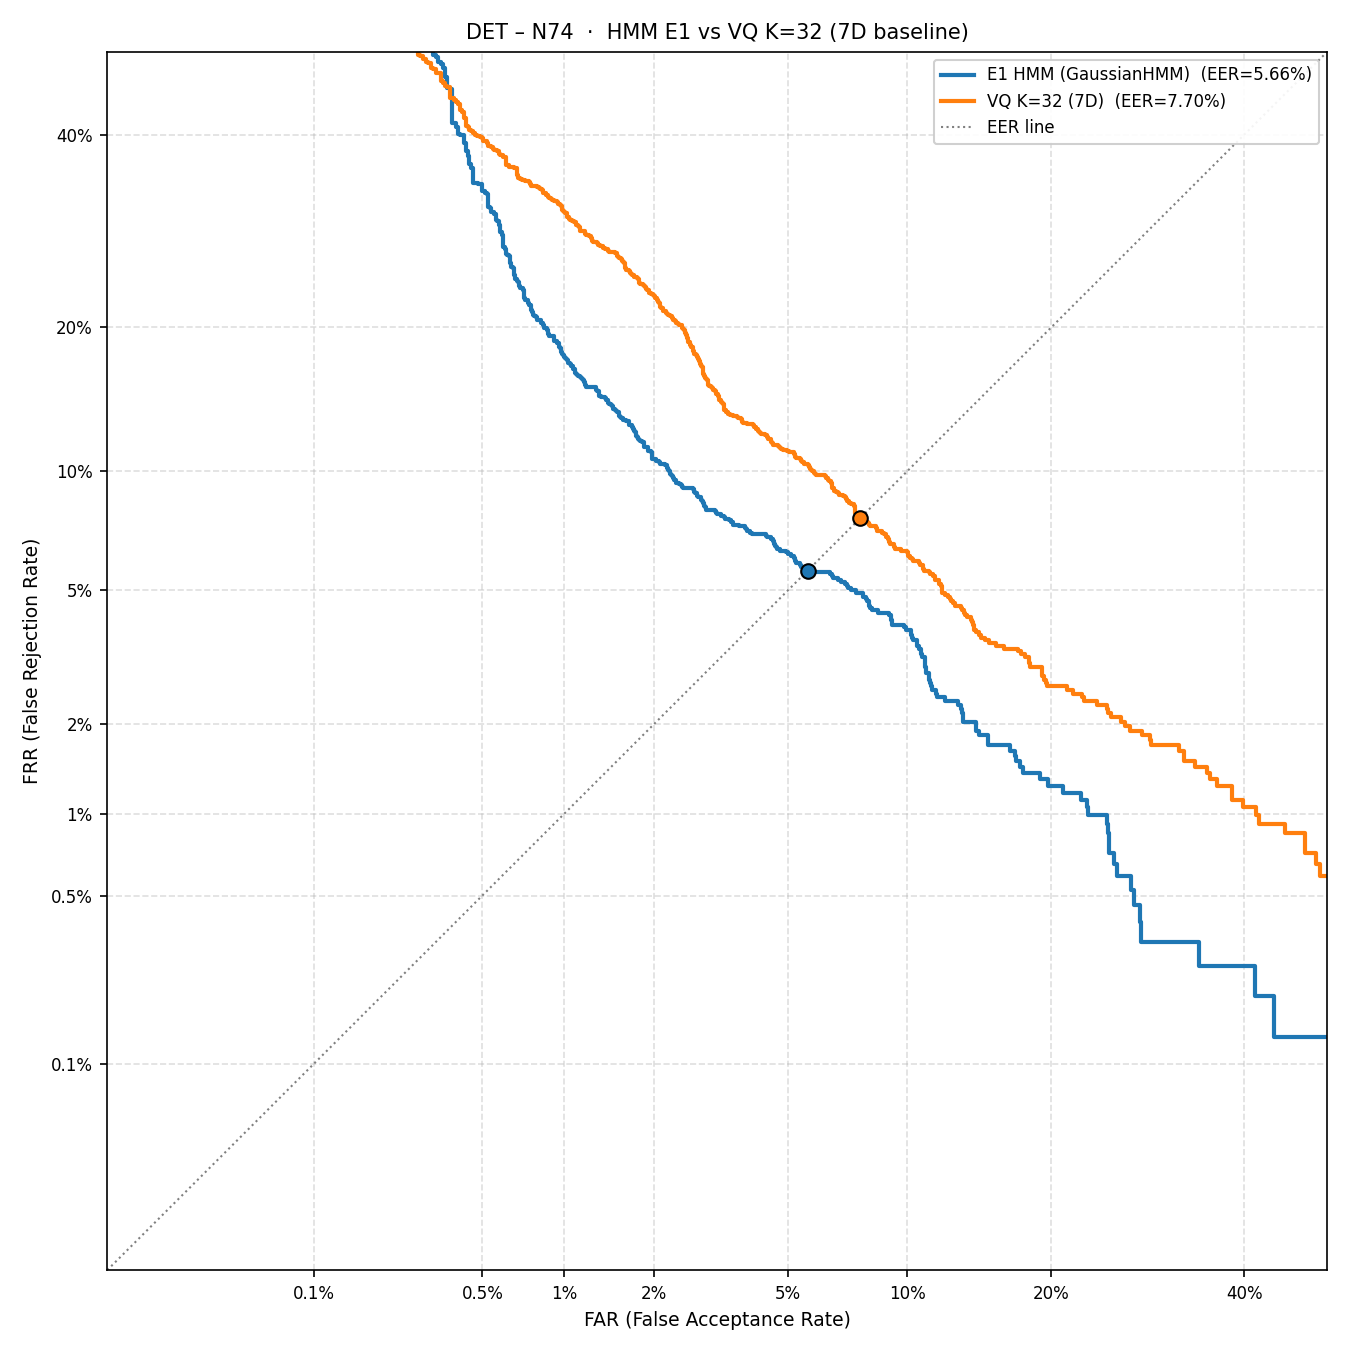
\includegraphics[width=0.65\textwidth, keepaspectratio]{plot1_N74.png}
  \caption{Curvas DET (N=74): HMM (E1) frente a VQ base (K=32, 7D).}
  \label{fig:det1}
\end{figure}
\begin{figure}[H]
  \centering
  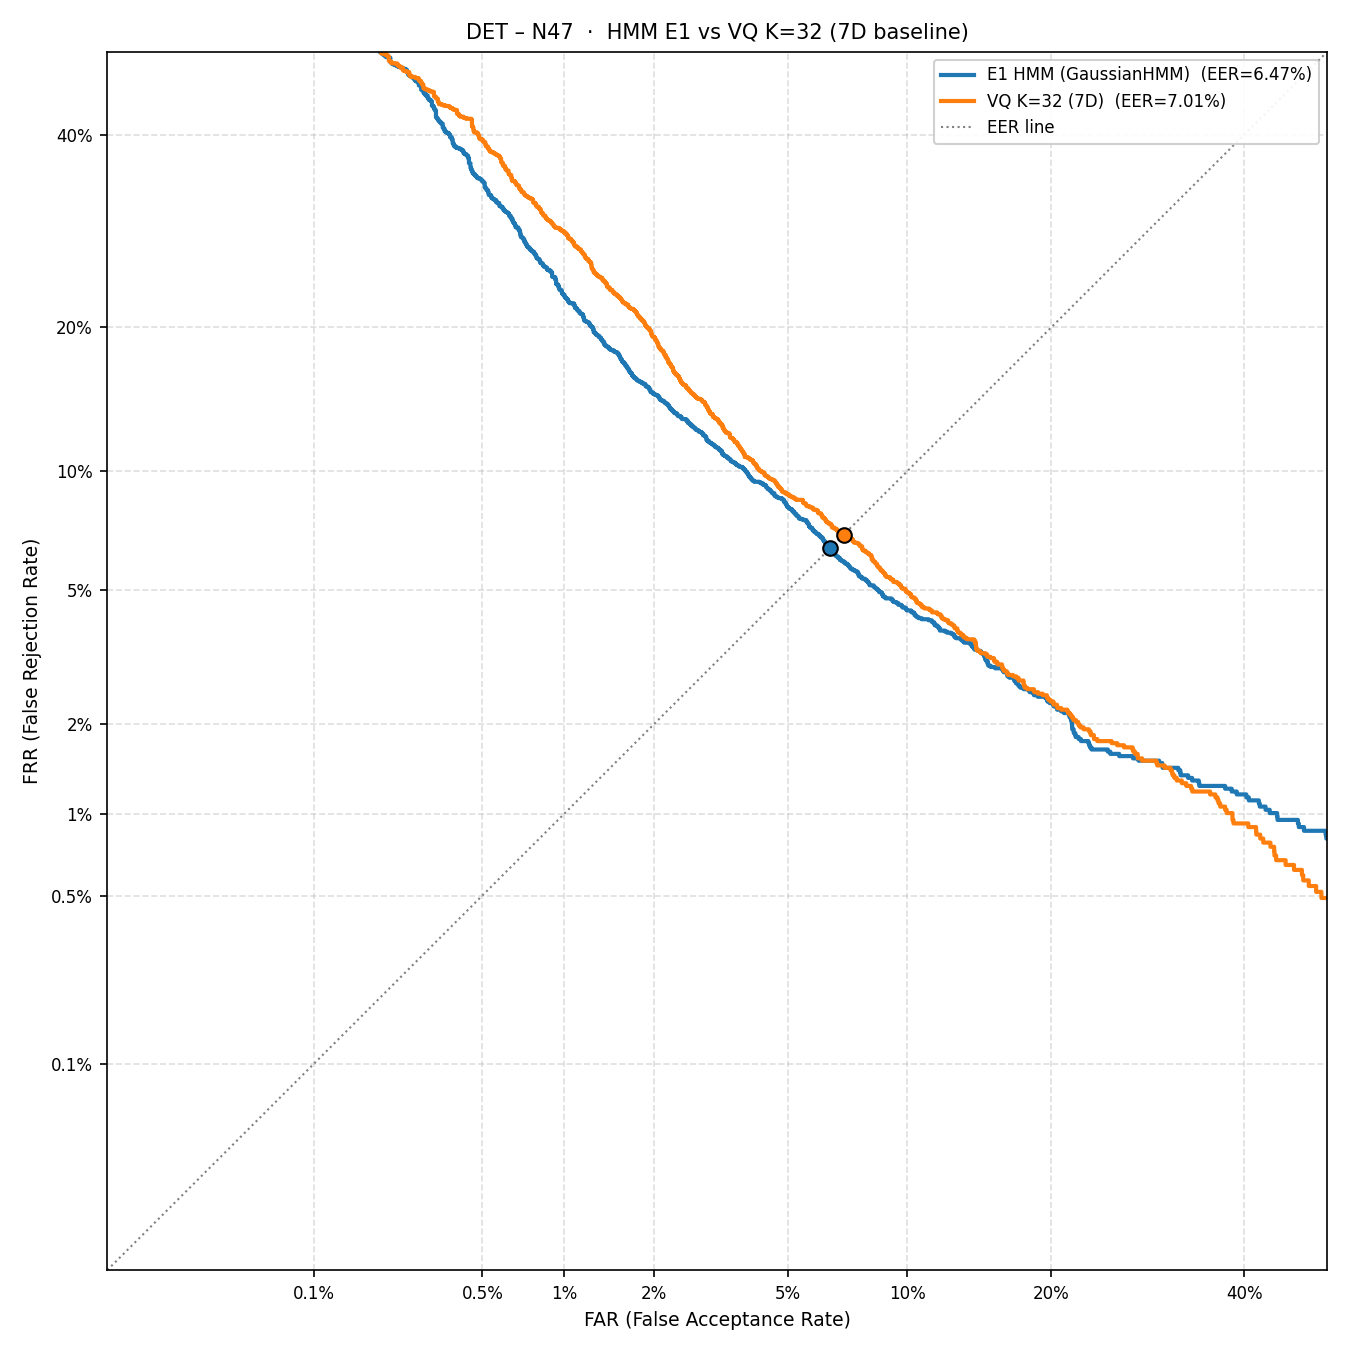
\includegraphics[width=0.65\textwidth, keepaspectratio]{plot1_N47.png}
  \caption{Curvas DET (N=47): HMM (E1) frente a VQ base (K=32, 7D).}
\end{figure}
\begin{figure}[H]
  \centering
  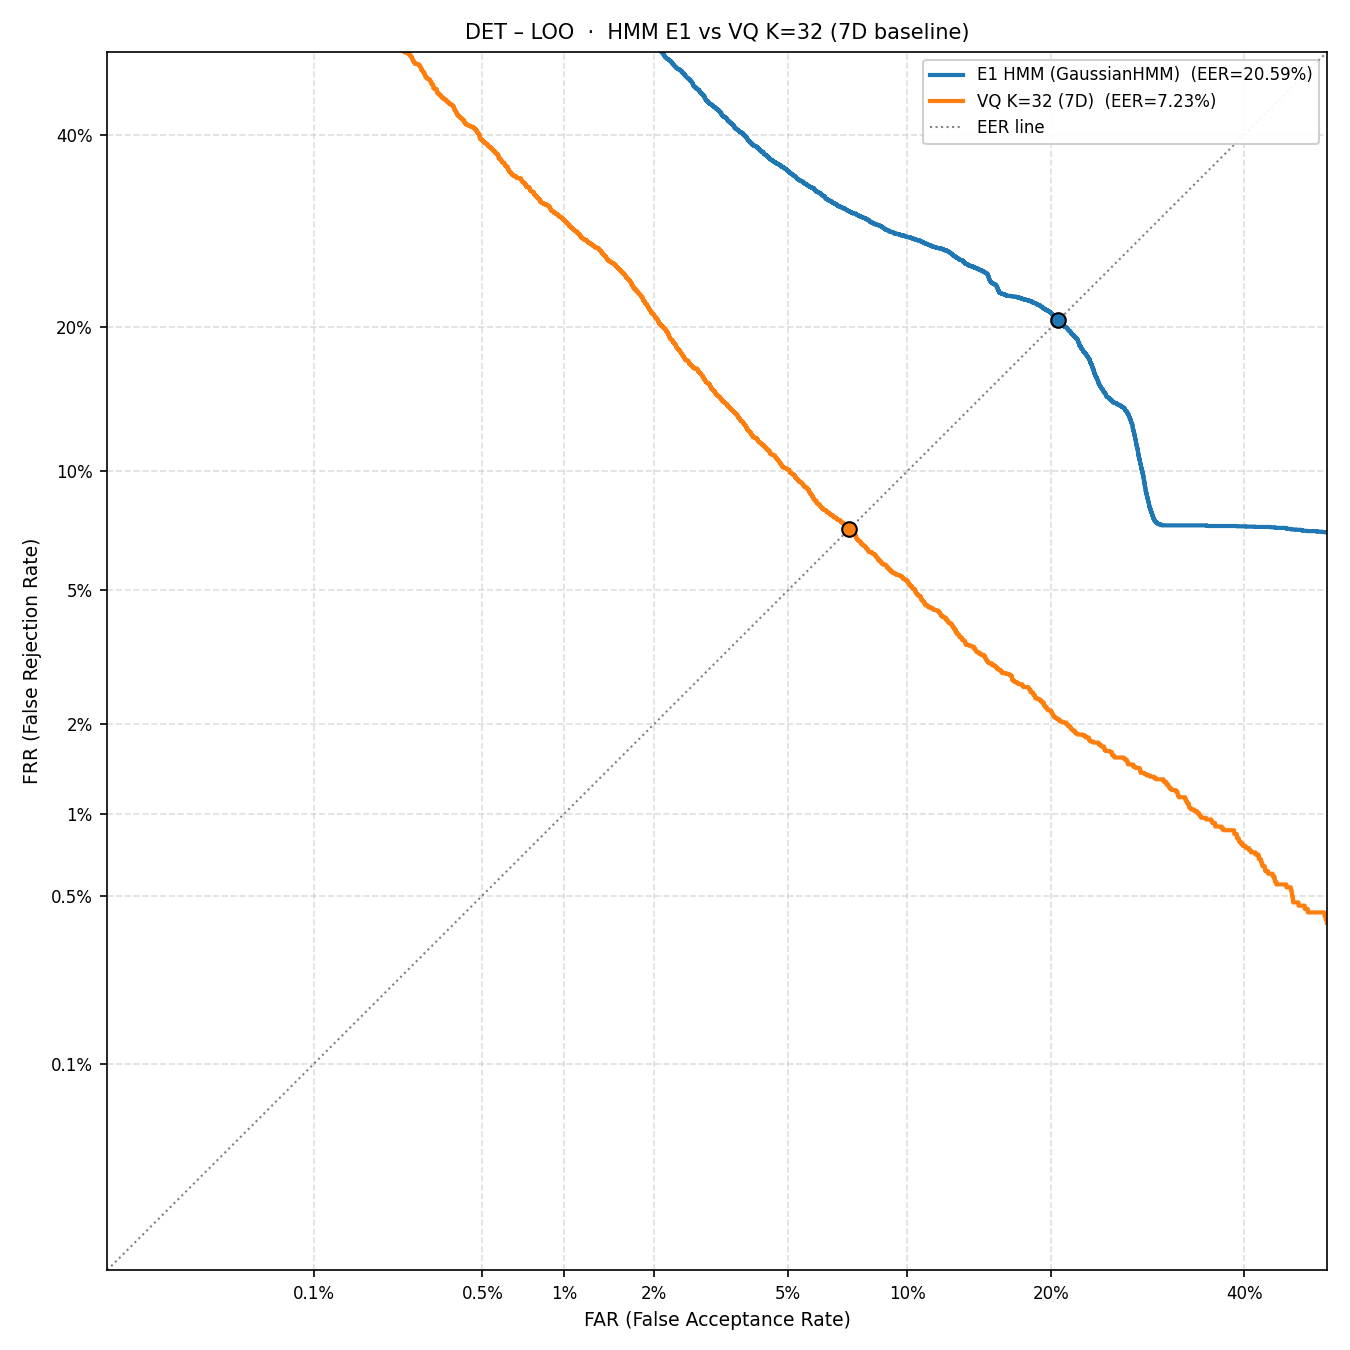
\includegraphics[width=0.65\textwidth, keepaspectratio]{plot1_LOO.png}
  \caption{Curvas DET (LOO): HMM (E1) frente a VQ base (K=32, 7D).}
\end{figure}

\subsection{Conclusiones del VQ}

El VQ es el sistema m\'{a}s eficiente en relaci\'{o}n a su coste: el entrenamiento
de un codebook por d\'{i}gito con MiniBatchKMeans tarda segundos, y sin embargo
obtiene el mejor EER individual del estudio (1.84--1.93\% seg\'{u}n el escenario).
La clave es la elecci\'{o}n de las caracter\'{i}sticas: el subconjunto de 5 dimensiones
orientado a posici\'{o}n y curvatura captura lo esencial del trazo manuscrito sin
ruido extra. El principal l\'{i}mite del VQ es que no modela la din\'{a}mica temporal
de la escritura; cada punto se trata de forma independiente, lo que impide
distinguir d\'{i}gitos que comparten formas locales pero difieren en el orden de
los trazos.

\newpage
% =============================================================================
\section{Modelos Ocultos de Markov (HMM)}
% =============================================================================

\subsection{Descripci\'{o}n del m\'{e}todo}

\textit{C\'{o}digo:} el HMM gaussiano simple (E1) est\'{a} en
\texttt{Entrega1/clasificador\_digitos.py} (preprocesado, extracci\'{o}n de
caracter\'{i}sticas y entrenamiento). El GMMHMM (E2) est\'{a} en
\texttt{Entrega2/HMM/clasificador\_digitos\_v3.py} (funci\'{o}n
\texttt{entrenar\_gmmhmm\_digito}).

Un HMM de izquierda a derecha modela la secuencia temporal de vectores de
caracter\'{i}sticas como una cadena de estados ocultos que solo puede avanzar hacia
la derecha o quedarse en el mismo estado (autolazos). Cada estado emite
vectores con una distribuci\'{o}n gaussiana. Para clasificar, se calcula la
log-verosimilitud de la secuencia bajo el modelo de cada d\'{i}gito y se elige
el d\'{i}gito con mayor verosimilitud.

En la Entrega 2 se pas\'{o} a un HMM con mezcla de Gaussianas por estado (GMMHMM),
lo que permite capturar distribuciones multimodales dentro de cada estado y
modelar con mayor precisi\'{o}n los distintos estilos de escritura.

El preprocesado de la trayectoria incluye suavizado Savitzky-Golay, remuestreo
equiespaciado en arco a 80 puntos, centrado y escalado a $[-1, 1]$, y
normalizaci\'{o}n Z-score sobre el conjunto de entrenamiento.

\subsection{Hiperpar\'{a}metros y variantes exploradas}

\textit{C\'{o}digo:} la b\'{u}squeda de hiperpar\'{a}metros del HMM E1 se
ejecuta desde \texttt{Entrega1/ejecutar\_parcial.py} y
\texttt{Entrega1/ejecutar\_loo.py}. La del GMMHMM (E2) est\'{a} integrada en
\texttt{Entrega2/HMM/clasificador\_digitos\_v3.py}.

Para el \textbf{HMM gaussiano simple (Entrega 1)} se realiz\'{o} una b\'{u}squeda sobre:

\begin{itemize}
  \item N\'{u}mero de estados: 3, 5, 7, 10 y 15.
  \item Tipo de covarianza: \texttt{full}, \texttt{diag}, \texttt{tied},
        \texttt{spherical}.
  \item Subconjunto de caracter\'{i}sticas: \texttt{min} (7D), \texttt{med} (12D)
        y \texttt{full} (21D).
  \item Probabilidad de autolazo: 0.3, 0.5, 0.6, 0.7 y 0.9.
\end{itemize}

La mejor configuraci\'{o}n result\'{o} ser 7 estados, covarianza diagonal,
subconjunto \texttt{med} (12D) y probabilidad de autolazo 0.6, alcanzando
una precisi\'{o}n del 92.9\% en N$=$74.

Para el \textbf{GMMHMM (Entrega 2)} se mantuvo la misma topolog\'{i}a y se
a\~{n}adi\'{o} la b\'{u}squeda sobre el n\'{u}mero de componentes por mezcla
(\texttt{n\_mix} $\in \{1, 2, 3\}$). La mejor configuraci\'{o}n fue
\texttt{n\_mix}$=$2 con el resto de hiperpar\'{a}metros iguales. Con entrenamiento
completo (100 iteraciones EM, 10 reinicios por d\'{i}gito) alcanz\'{o} un 93.0\% en
N$=$74 y un 93.3\% en N$=$47, con EER de 3.09\% y 4.78\% respectivamente.

\subsection{Resultados}

\begin{table}[H]
  \centering
  \caption{Precisi\'{o}n (\%) y EER (\%) de los sistemas HMM.}
  \label{tab:hmm}
  \begin{tabular}{lcccccc}
    \toprule
    & \multicolumn{2}{c}{\textbf{N=74}} & \multicolumn{2}{c}{\textbf{N=47}}
    & \multicolumn{2}{c}{\textbf{LOO}} \\
    \cmidrule(lr){2-3}\cmidrule(lr){4-5}\cmidrule(lr){6-7}
    \textbf{Sistema} & Acc. & EER & Acc. & EER & Acc. & EER \\
    \midrule
    HMM gaussiano (E1) & 92.9 & 5.66 & 89.8 & 6.47 & n.a. & 20.59 \\
    GMMHMM (E2, bien entrenado) & 93.0 & 3.09 & 93.3 & 4.78 & 80.5$^{*}$ & 17.38$^{*}$ \\
    \bottomrule
  \end{tabular}

  \smallskip
  \small $^{*}$ El LOO del GMMHMM se realiz\'{o} con 5-fold y par\'{a}metros reducidos
  (80 iter., 6 reinicios); ver texto.
\end{table}

La Figura~\ref{fig:det2} a\~{n}ade el GMMHMM y el VQ optimizado a las curvas de
la secci\'{o}n anterior, permitiendo comparar los cuatro sistemas base.

\begin{figure}[H]
  \centering
  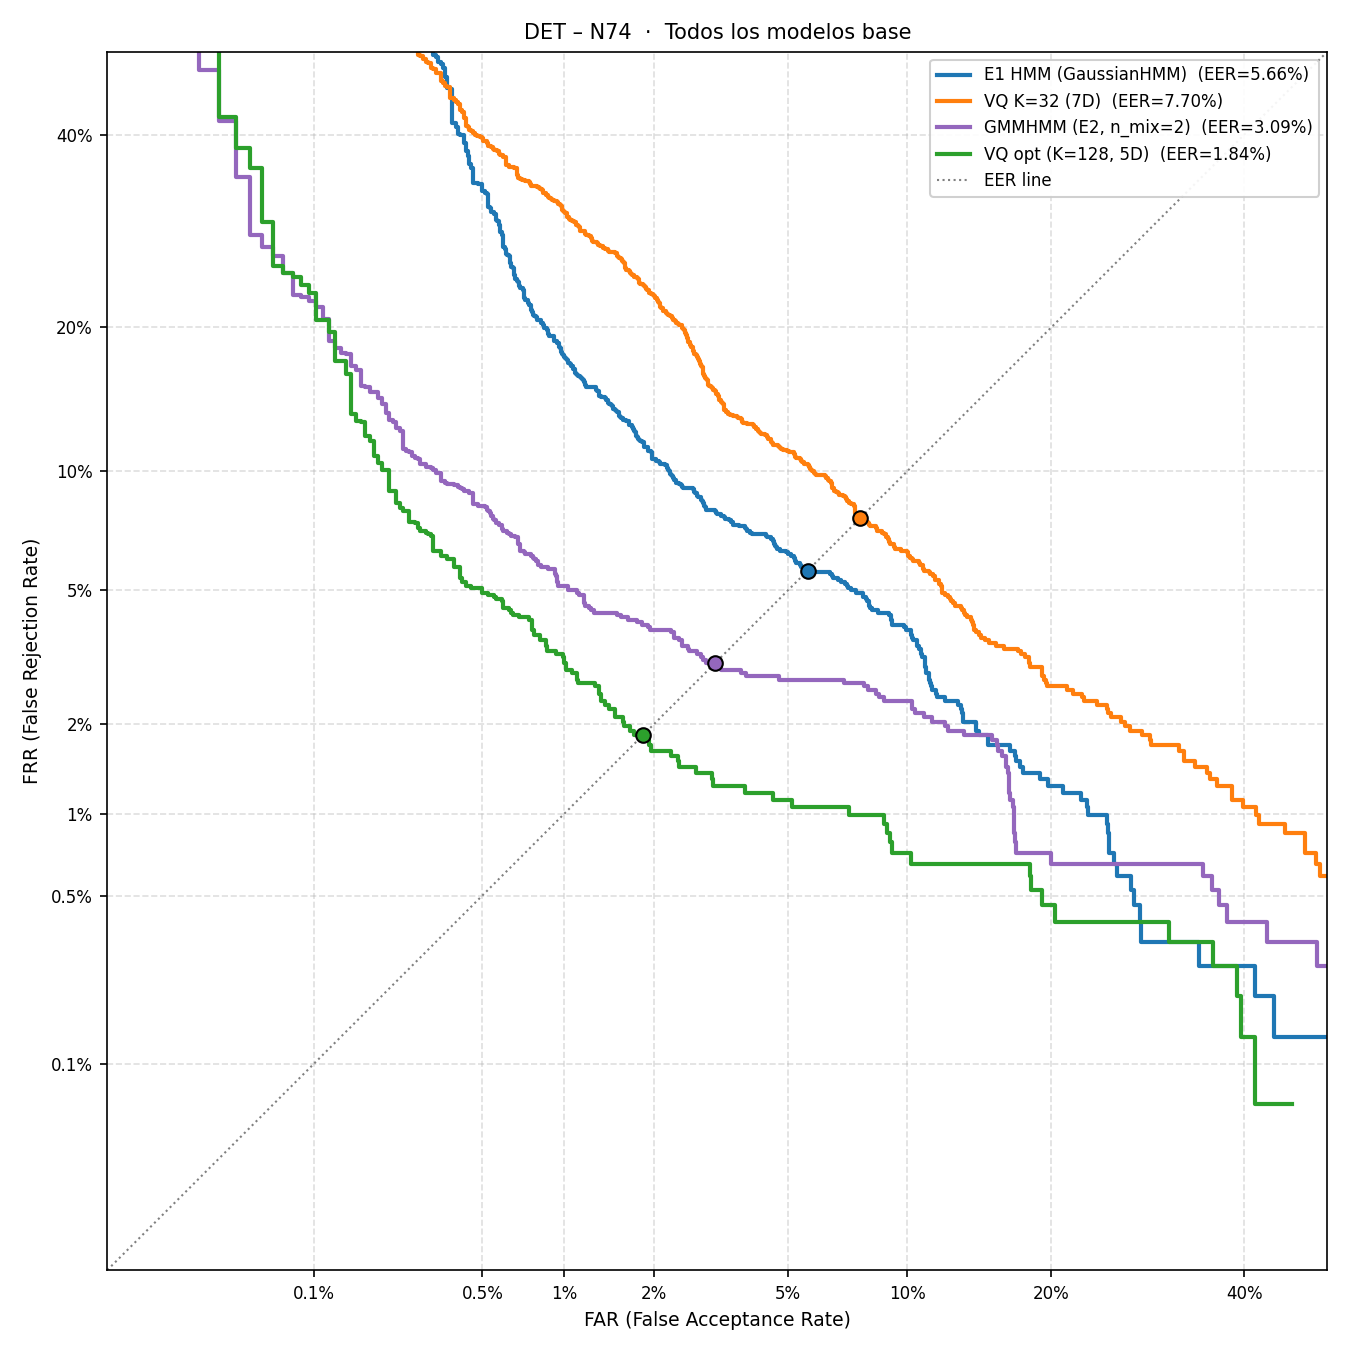
\includegraphics[width=0.65\textwidth, keepaspectratio]{plot2_N74.png}
  \caption{Curvas DET (N=74): todos los modelos individuales.}
  \label{fig:det2}
\end{figure}
\begin{figure}[H]
  \centering
  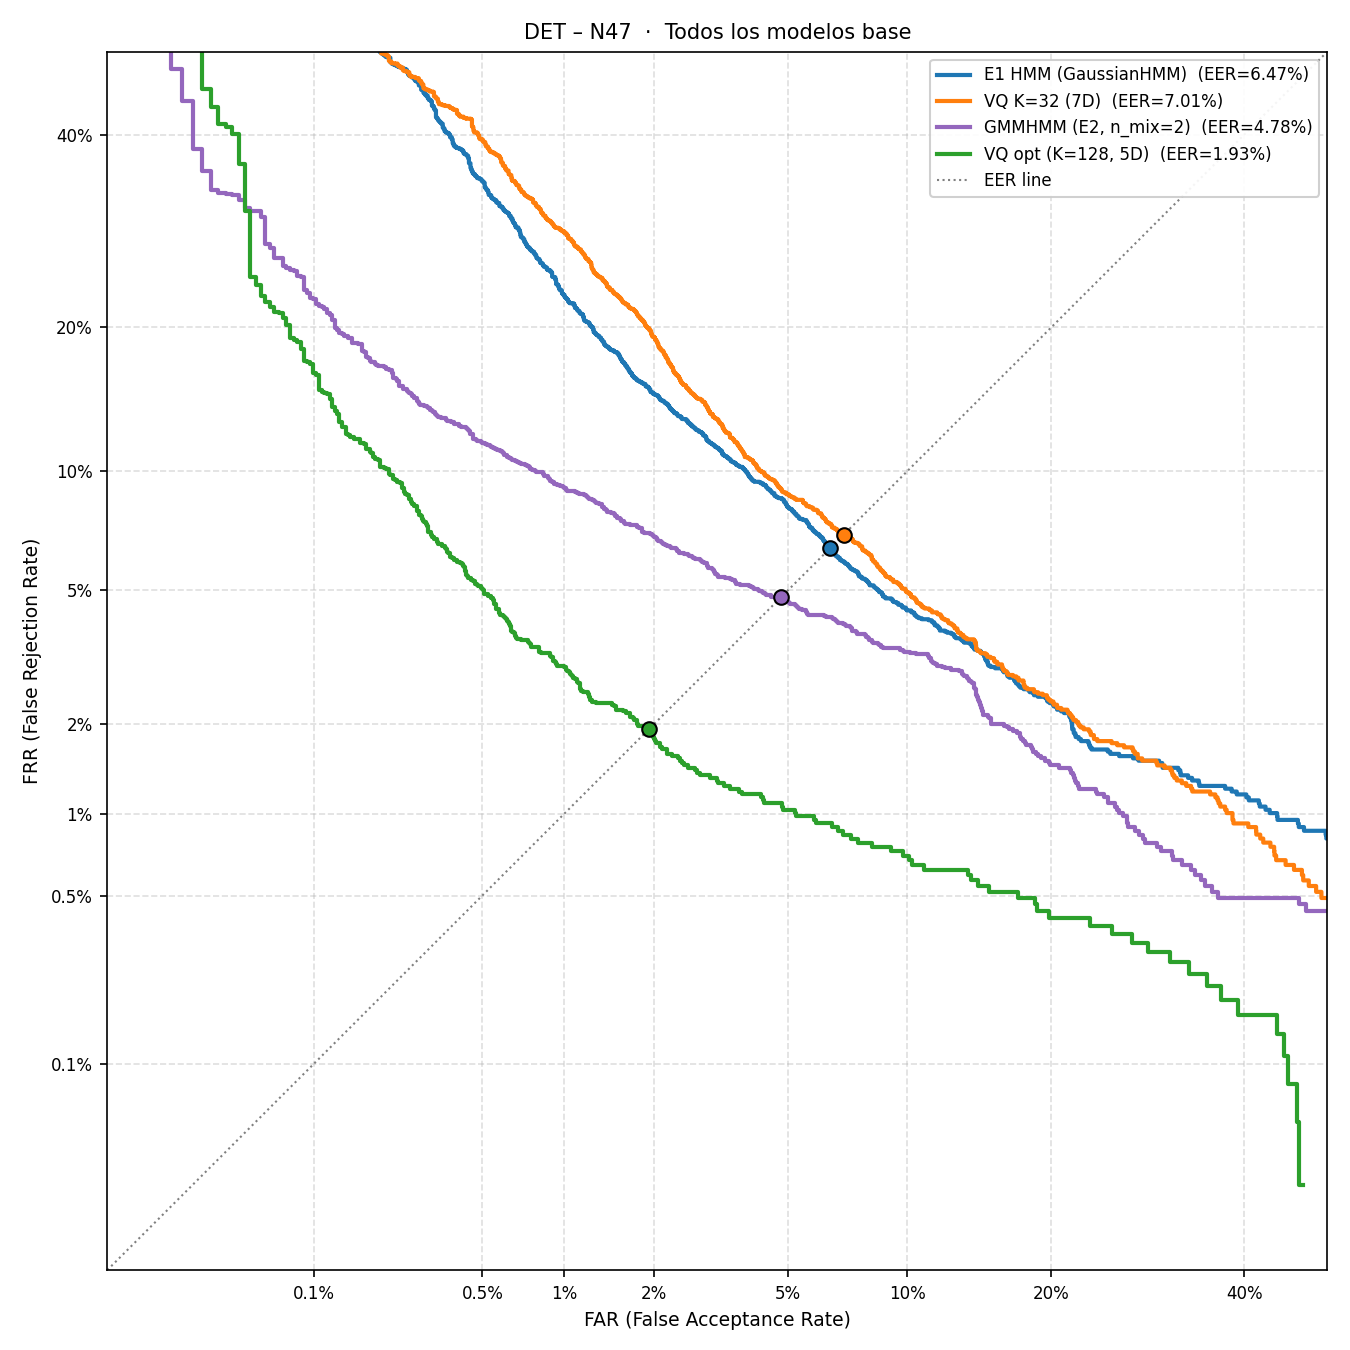
\includegraphics[width=0.65\textwidth, keepaspectratio]{plot2_N47.png}
  \caption{Curvas DET (N=47): todos los modelos individuales.}
\end{figure}
\begin{figure}[H]
  \centering
  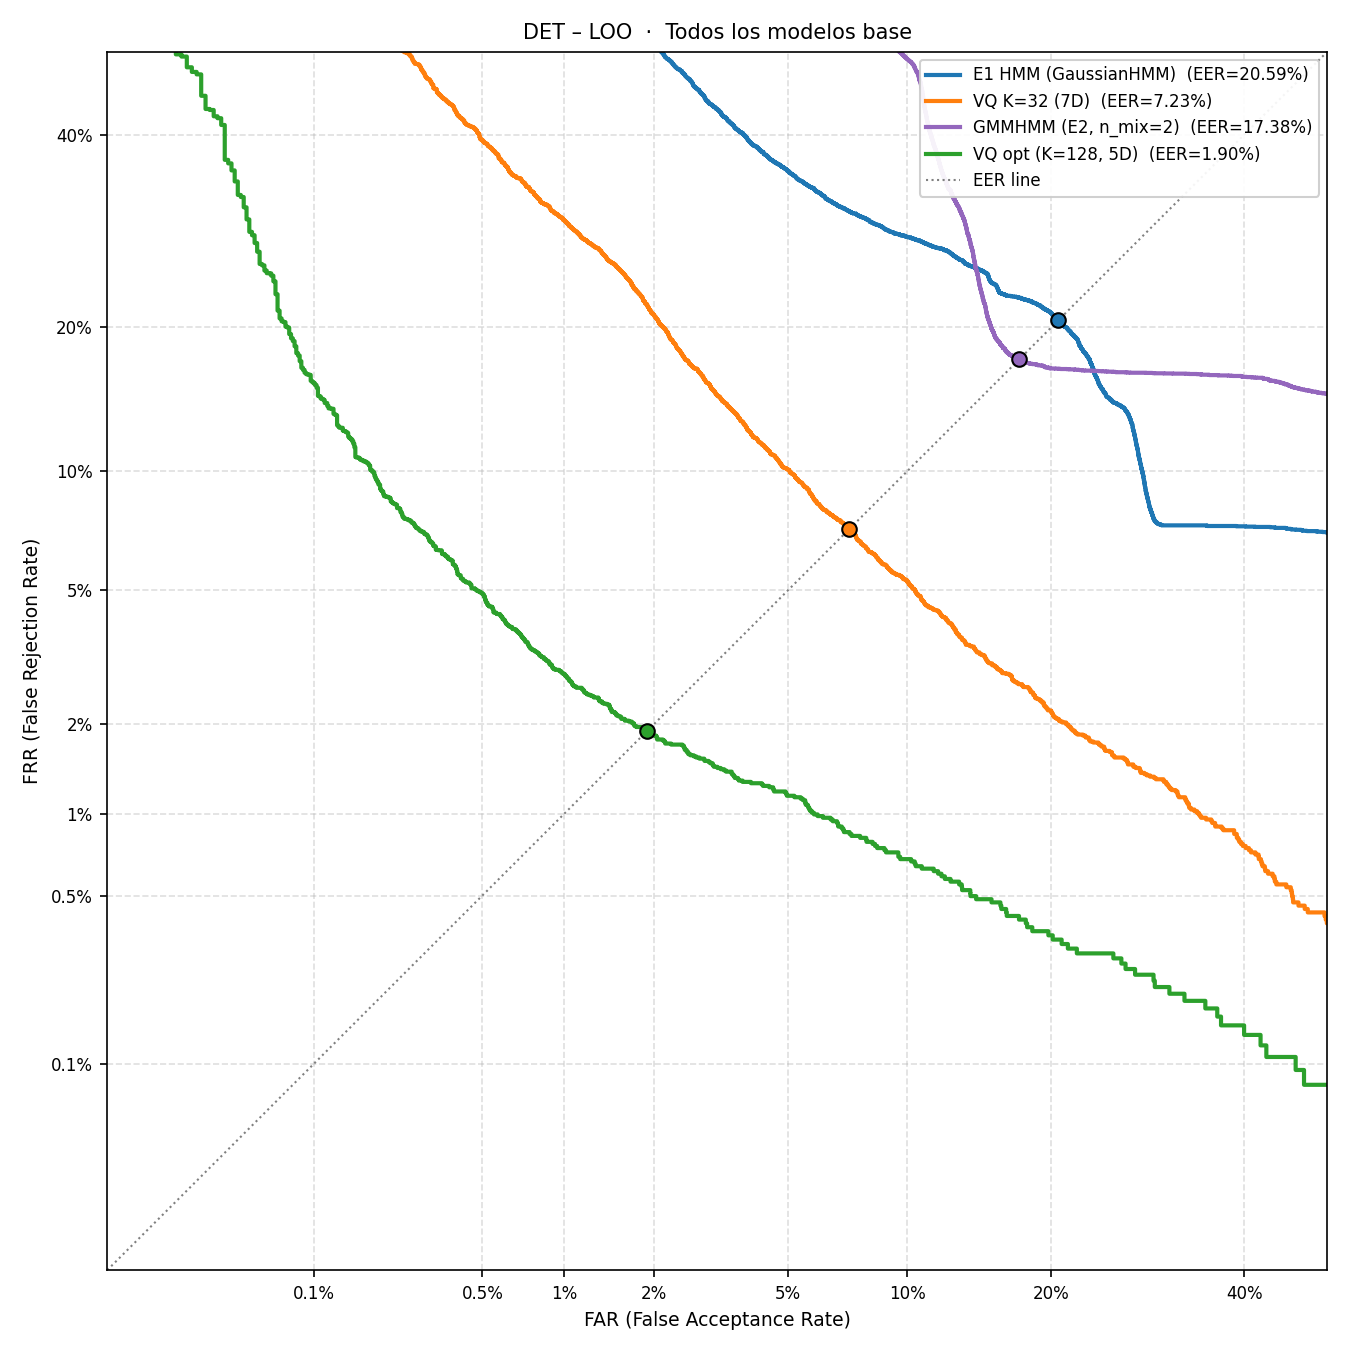
\includegraphics[width=0.65\textwidth, keepaspectratio]{plot2_LOO.png}
  \caption{Curvas DET (LOO): todos los modelos individuales.}
\end{figure}

\subsection{El coste computacional del GMMHMM y el LOO}

\textit{C\'{o}digo:} el reentrenamiento completo del GMMHMM (100 iter., 10
reinicios) para los escenarios N$=$74 y N$=$47 se hace en
\texttt{Entrega3/train\_hmm\_vq\_splits.py}, que guarda los resultados en
\texttt{Entrega3/Paralel/resultados/ensemble\_\{N74,N47\}\_full.json}.
La aproximaci\'{o}n K5-fold del LOO est\'{a} en
\texttt{Entrega3/kfold\_hmm\_vq.py} (salida en
\texttt{ensemble\_K5fold.json}).

El algoritmo EM del GMMHMM converge de forma significativamente m\'{a}s lenta que
el del HMM gaussiano simple. En la m\'{a}quina de trabajo, entrenar los 10 modelos
(uno por d\'{i}gito) con 100 iteraciones y 10 reinicios requiere aproximadamente
\textbf{6 horas para N$=$74}. El LOO cl\'{a}sico implicar\'{i}a repetir esto 93 veces,
lo que supone unas 444 horas (18 d\'{i}as), un coste inasumible.

Como alternativa, se utiliz\'{o} una validaci\'{o}n cruzada con \textbf{5 pliegues por
usuario} (K5-fold), que reduce el n\'{u}mero de entrenamientos a 5. Con par\'{a}metros
algo m\'{a}s ajustados (80 iter., 6 reinicios) el tiempo total baj\'{o} a unas 14--15
horas. El resultado del LOO aproximado (80.5\% de precisi\'{o}n) es inferior al de
N$=$74 porque cada fold dispone de menos datos de entrenamiento relativos y porque
los par\'{a}metros de entrenamiento son m\'{a}s limitados.

\subsection{Conclusiones del HMM}

El GMMHMM mejora claramente al HMM gaussiano simple cuando se entrena con los
recursos adecuados. La mejora en EER respecto al HMM de la Entrega 1 es notable
en los escenarios con conjunto de entrenamiento fijo (N$=$74 y N$=$47). Sin embargo,
el VQ optimizado sigue siendo superior en todos los escenarios, incluso siendo
un modelo mucho m\'{a}s simple. El HMM a\~{n}ade valor al sistema por una raz\'{o}n
distinta: sus errores no coinciden exactamente con los del VQ, lo que abre la
puerta a combinaciones en ensemble que pueden superar a cualquiera de los dos
por separado.

\newpage
% =============================================================================
\section{Sistemas en Ensemble}
% =============================================================================

\subsection{Motivaci\'{o}n: el HMM y el VQ se equivocan de forma distinta}

\textit{C\'{o}digo:} el scatter por usuario se genera en
\texttt{Entrega2/comparacion/} (al comparar HMM y VQ por usuario).

Antes de describir los ensembles conviene ver si tiene sentido combinar HMM y VQ.
La Figura~\ref{fig:scatter} muestra la precisi\'{o}n por usuario de ambos sistemas
en el escenario N$=$74. Cada punto es un usuario de test; el eje horizontal
recoge la precisi\'{o}n del HMM y el vertical la del VQ.

\begin{figure}[H]
  \centering
  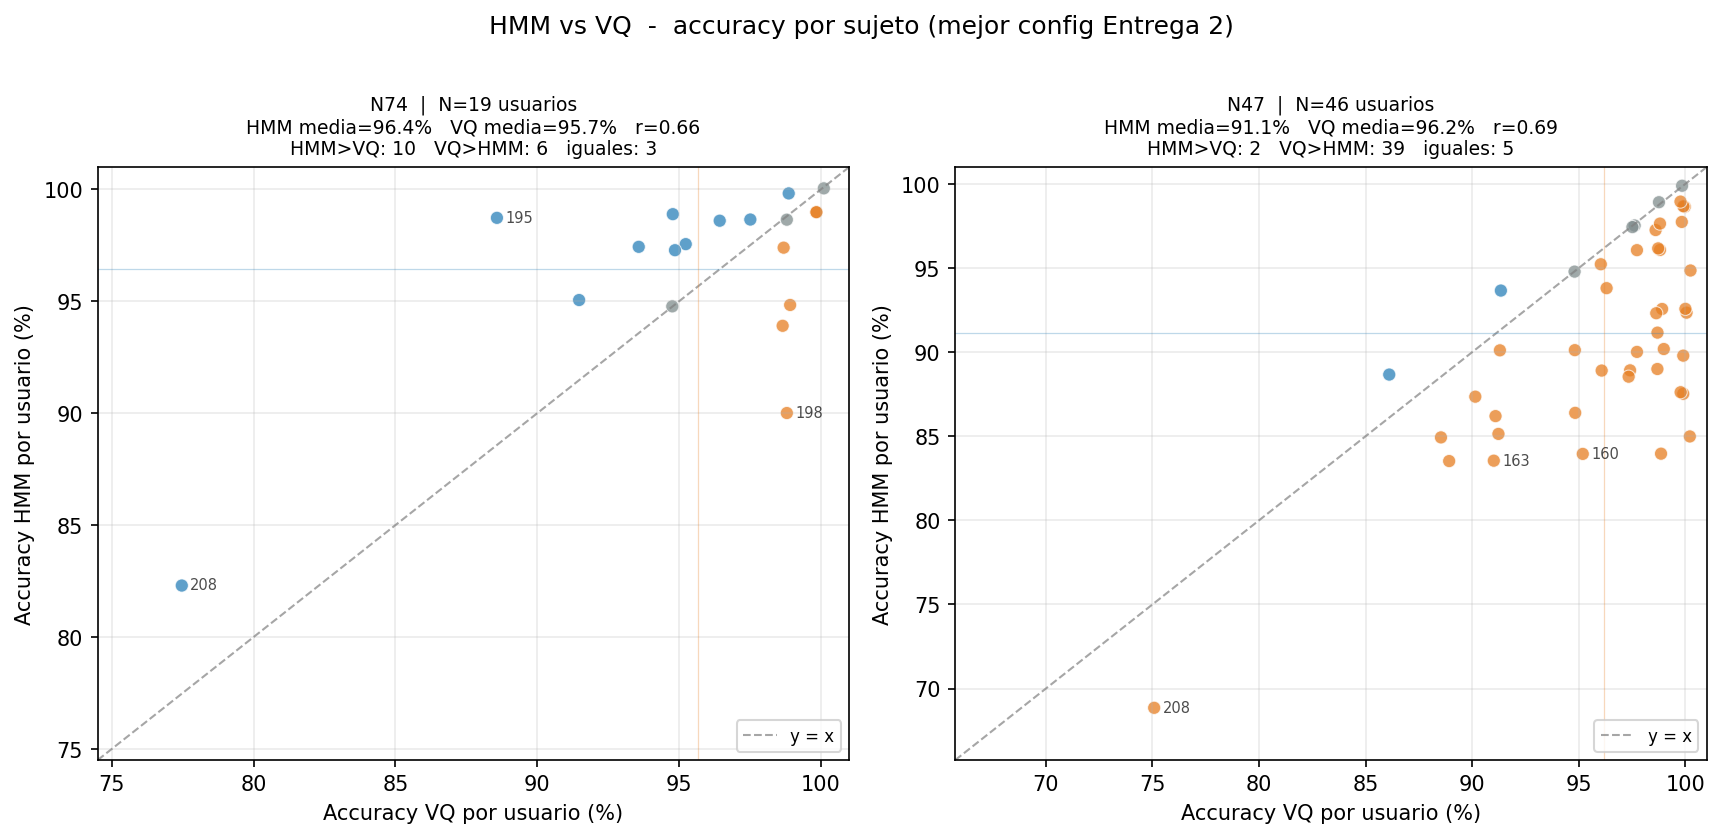
\includegraphics[width=\textwidth, keepaspectratio]{scatter_por_usuario.png}
  \caption{Precisi\'{o}n por usuario: HMM (eje X) frente a VQ (eje Y) en N$=$74.
           Los puntos fuera de la diagonal indican usuarios en los que un
           modelo acierta y el otro falla.}
  \label{fig:scatter}
\end{figure}

Si ambos modelos cometieran los mismos errores, los puntos estar\'{i}an sobre la
diagonal y no habr\'{i}a nada que ganar combin\'{a}ndolos. El hecho de que existan
puntos alejados de la diagonal indica que hay usuarios para los que el HMM
falla pero el VQ acierta (y viceversa). Esto sugiere que una combinaci\'{o}n
inteligente puede recuperar parte de esos errores.

El hecho de que los errores de ambos modelos no coincidan implica que existe
margen real para mejorar combinando sus predicciones.

\subsection{Ensemble paralelo}

\textit{C\'{o}digo:} el ensemble paralelo con sus reglas de fusi\'{o}n
(\texttt{agreement}, \texttt{soft}, \texttt{conf\_weighted},
\texttt{margin\_weighted}) est\'{a} en
\texttt{Entrega3/Paralel/ensemble\_paralelo.py}. La versi\'{o}n con el
GMMHMM bien entrenado se obtiene en
\texttt{Entrega3/train\_hmm\_vq\_splits.py}.

En el ensemble paralelo, el HMM y el VQ clasifican cada muestra de forma
independiente y sus puntuaciones se fusionan seg\'{u}n distintas reglas:

\begin{description}
  \item[\texttt{agreement}:] si ambos modelos coinciden, se usa esa predicci\'{o}n;
       si no, se elige el modelo con mayor confianza en la clase top-1.
  \item[\texttt{soft}:] promedio simple de las probabilidades softmax de ambos
       modelos, normalizadas por muestra para hacer las escalas comparables.
  \item[\texttt{conf\_weighted}:] ponderaci\'{o}n por la confianza top-1 de cada
       modelo (el que est\'{a} m\'{a}s seguro tiene m\'{a}s peso).
  \item[\texttt{margin\_weighted}:] ponderaci\'{o}n por el margen entre la clase
       m\'{a}s probable y la segunda, que refleja mejor cu\'{a}nto se destaca la
       decisi\'{o}n de cada modelo.
\end{description}

La regla \texttt{margin\_weighted} es la que consigue mejores resultados en todos
los escenarios; es tambi\'{e}n la \'{u}nica que no requiere informaci\'{o}n futura
(a diferencia del or\'{a}culo, que conoce las etiquetas reales).

\begin{table}[H]
  \centering
  \caption{Precisi\'{o}n (\%) y EER (\%) del ensemble paralelo (\texttt{margin\_weighted}).}
  \label{tab:par}
  \begin{tabular}{lcccccc}
    \toprule
    & \multicolumn{2}{c}{\textbf{N=74}} & \multicolumn{2}{c}{\textbf{N=47}}
    & \multicolumn{2}{c}{\textbf{LOO (K5)}} \\
    \cmidrule(lr){2-3}\cmidrule(lr){4-5}\cmidrule(lr){6-7}
    \textbf{Sistema} & Acc. & EER & Acc. & EER & Acc. & EER \\
    \midrule
    Paralelo margin\_weighted & 97.6 & 1.69 & 97.3 & 1.74 & 97.0 & 2.30 \\
    \bottomrule
  \end{tabular}
\end{table}

\subsection{Ensemble serial}

\textit{C\'{o}digo:} la cascada serial original (HMM $\to$ VQ en espacio
LL) est\'{a} en \texttt{Entrega3/Serial/serial\_hmm\_vq.py}. La actualizaci\'{o}n
con el GMMHMM bien entrenado se hace con
\texttt{Entrega3/Serial/update\_serial\_full\_hmm.py}. La cascada serial
VQ-dominante est\'{a} implementada como funci\'{o}n
\texttt{serial\_vq\_dominant} en
\texttt{Entrega3/generar\_det\_nuevos.py}.

En la cascada serial original (Entrega 3), el HMM genera un vector de
10 log-verosimilitudes que se usa como entrada a un clasificador VQ en ese
espacio de 10 dimensiones. La idea es que si el HMM funciona bien, la dimensi\'{o}n
correspondiente al d\'{i}gito correcto tendr\'{a} el valor m\'{a}s alto, y el VQ
aprender\'{a} esos patrones. Aun cuando se utiliza el GMMHMM bien entrenado
(100 iteraciones, 10 reinicios), la cadena resulta poco fiable: el VQ en el
espacio de log-verosimilitudes degrada respecto al baseline del propio HMM,
con EER del 11.5\% en N$=$74 y el 13.1\% en N$=$47. El motivo es que el VQ
no a\~{n}ade informaci\'{o}n nueva sobre las propias verosimilitudes y, al
introducir un modelo intermedio entrenado, propaga sus errores en lugar de
corregirlos.

Para mejorar este resultado se dise\~{n}\'{o} una \textbf{cascada VQ-dominante}: el VQ
act\'{u}a como primera etapa y el HMM solo contribuye en las muestras en las que el
VQ est\'{a} inseguro. Concretamente:

\begin{enumerate}
  \item Se calcula la distribuci\'{o}n de probabilidad del VQ sobre las 10 clases.
  \item Se mide la incertidumbre del VQ combinando su entrop\'{i}a normalizada y la
        falta de margen entre la clase m\'{a}s probable y la segunda.
  \item El score final es $\alpha \cdot p_\text{VQ} + (1-\alpha) \cdot p_\text{HMM}$,
        donde $\alpha \in [0.80,\, 1.00]$ crece con la confianza del VQ.
  \item El HMM nunca aporta m\'{a}s de un 20\% del peso total.
\end{enumerate}

Con esta estrategia el EER del serial baja hasta el 1.73\% en N$=$74 y el 1.66\%
en N$=$47, superando al VQ base (K$=$32, 7D) y acercando el serial al ensemble
paralelo.

\begin{table}[H]
  \centering
  \caption{Comparativa EER (\%) de todos los sistemas de ensemble.}
  \label{tab:ens}
  \begin{tabular}{lccc}
    \toprule
    \textbf{Sistema} & \textbf{N=74} & \textbf{N=47} & \textbf{LOO (K5)} \\
    \midrule
    Serial original (HMM $\to$ VQ en espacio LL) & 11.46 & 13.05 & 12.34 \\
    Serial VQ-dominante                           &  1.73 &  1.66 &  1.94 \\
    Paralelo margin\_weighted                     &  1.69 &  1.74 &  2.30 \\
    \bottomrule
  \end{tabular}
\end{table}

La Figura~\ref{fig:det3} muestra las curvas DET de los tres sistemas de ensemble.

\begin{figure}[H]
  \centering
  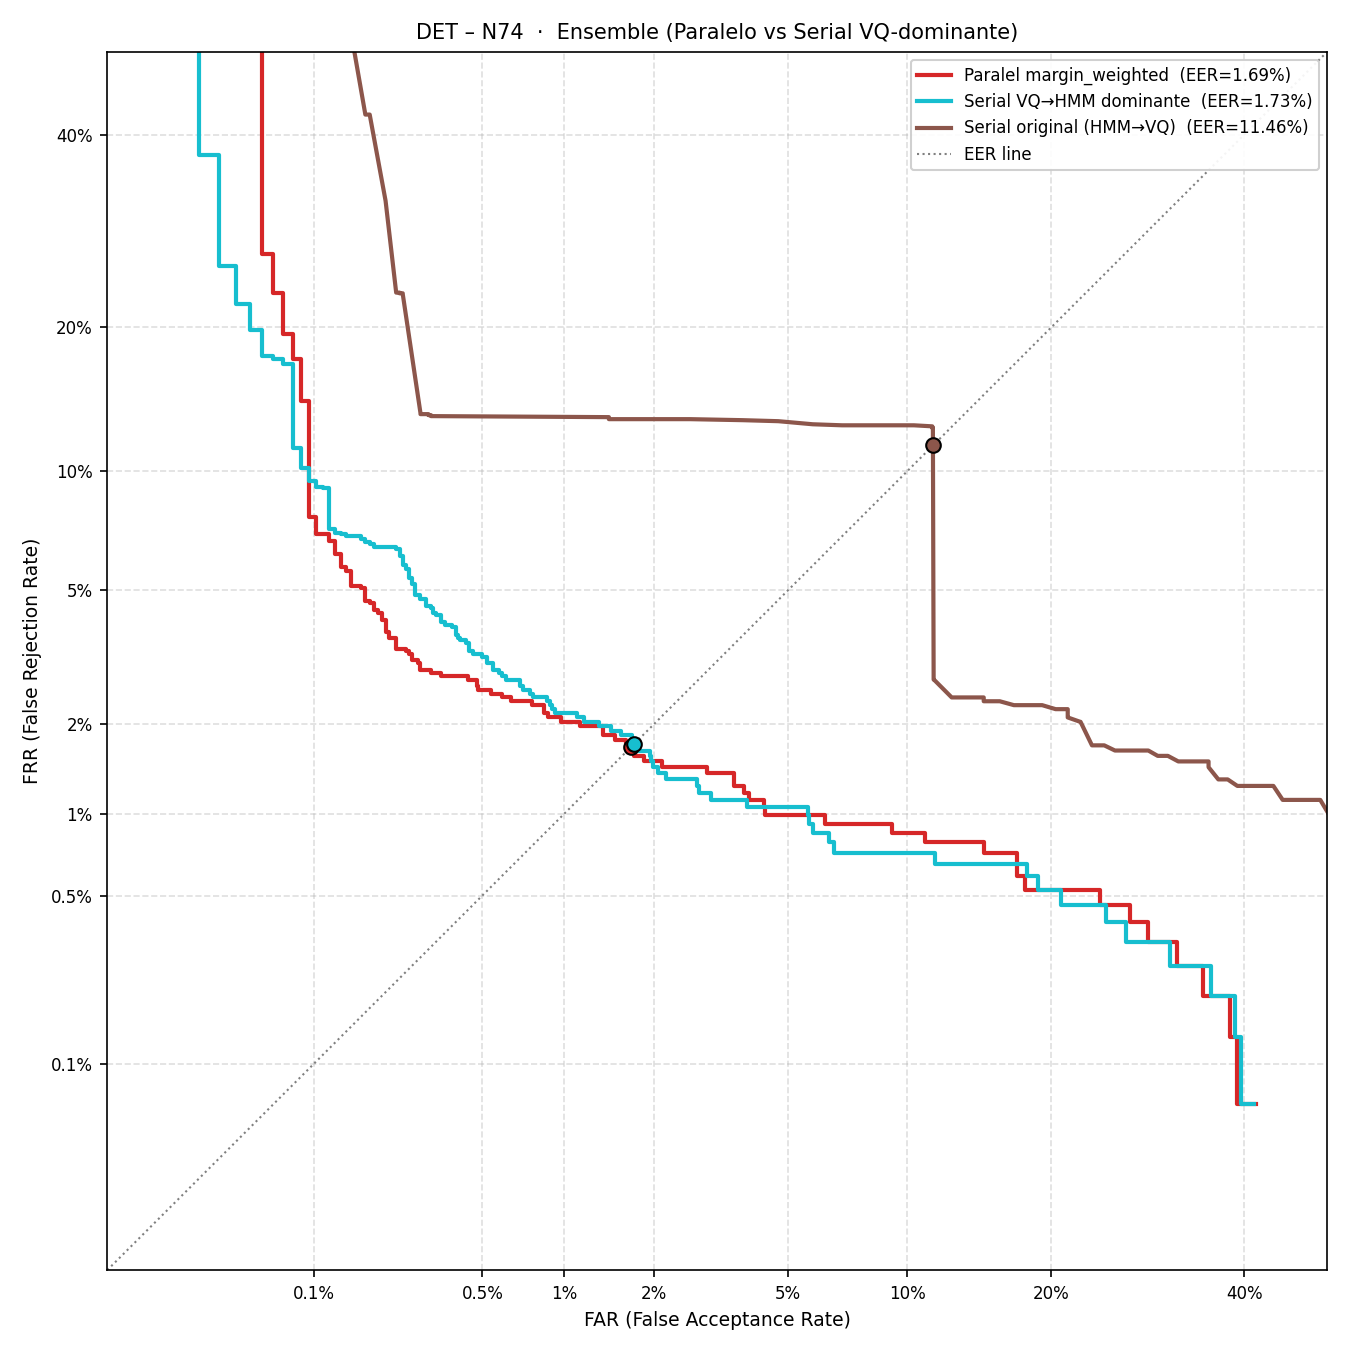
\includegraphics[width=0.65\textwidth, keepaspectratio]{plot3_N74.png}
  \caption{Curvas DET (N=74): sistemas en ensemble.}
  \label{fig:det3}
\end{figure}
\begin{figure}[H]
  \centering
  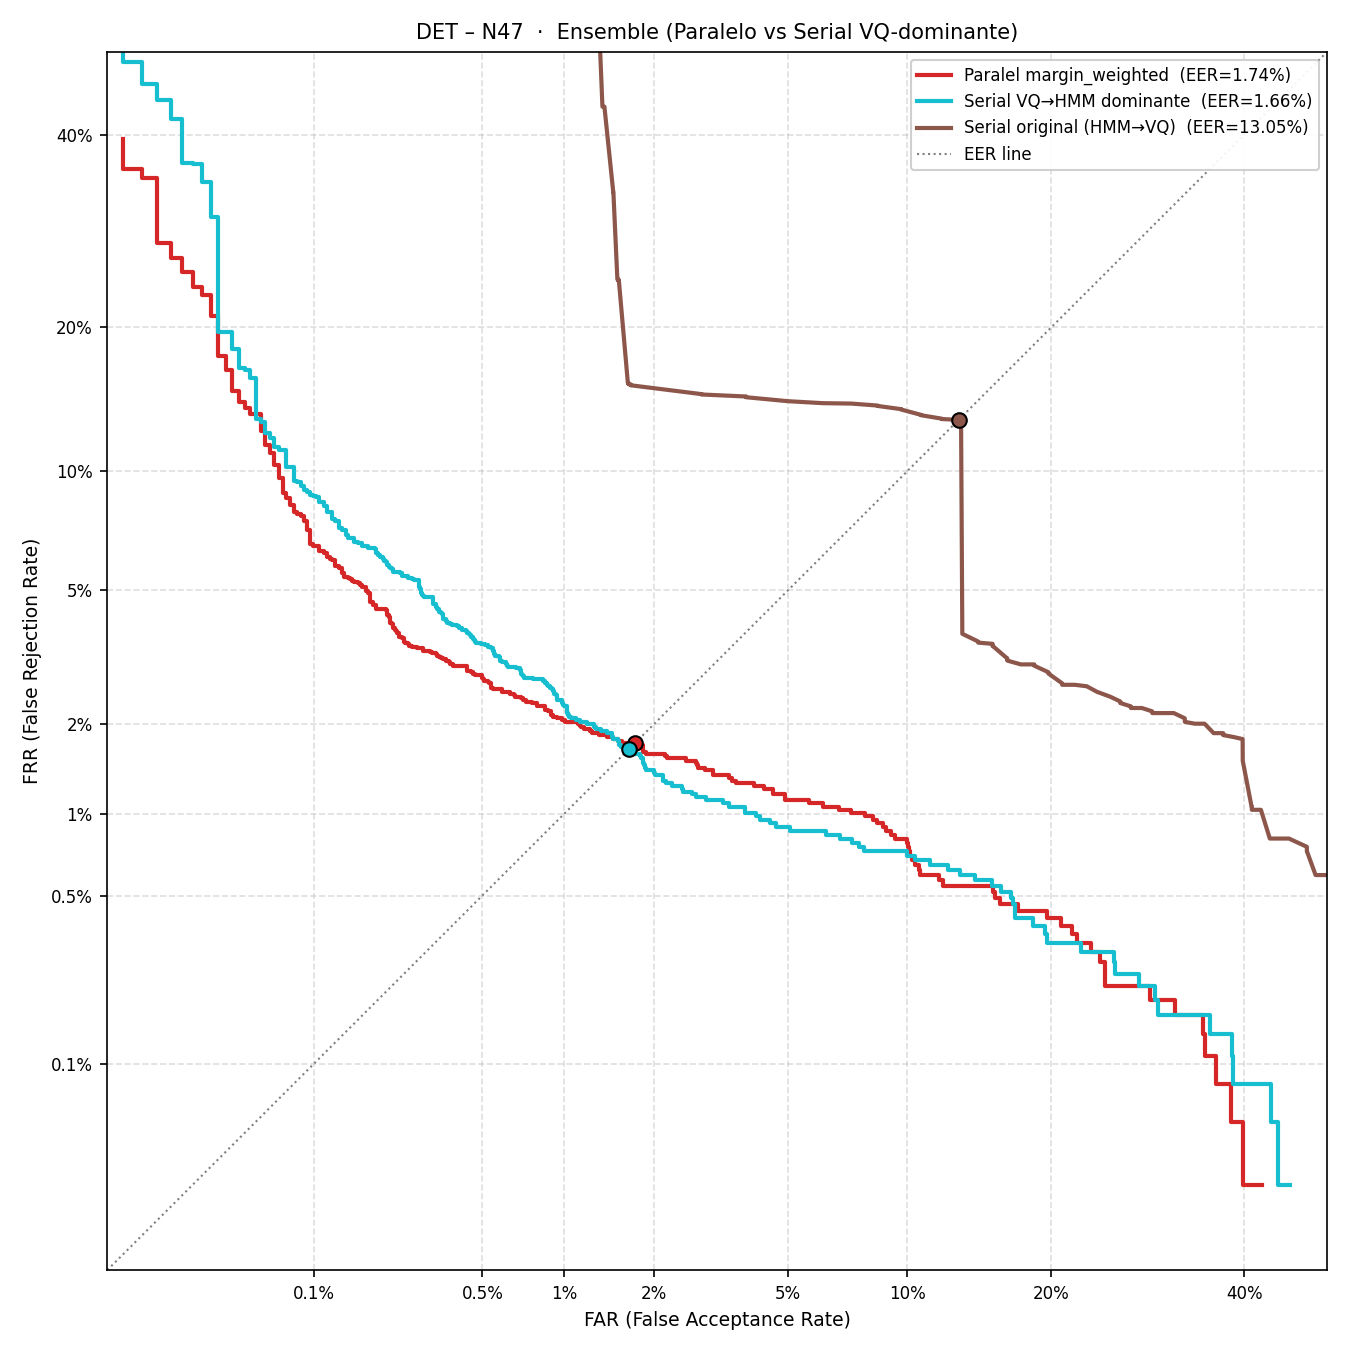
\includegraphics[width=0.65\textwidth, keepaspectratio]{plot3_N47.png}
  \caption{Curvas DET (N=47): sistemas en ensemble.}
\end{figure}
\begin{figure}[H]
  \centering
  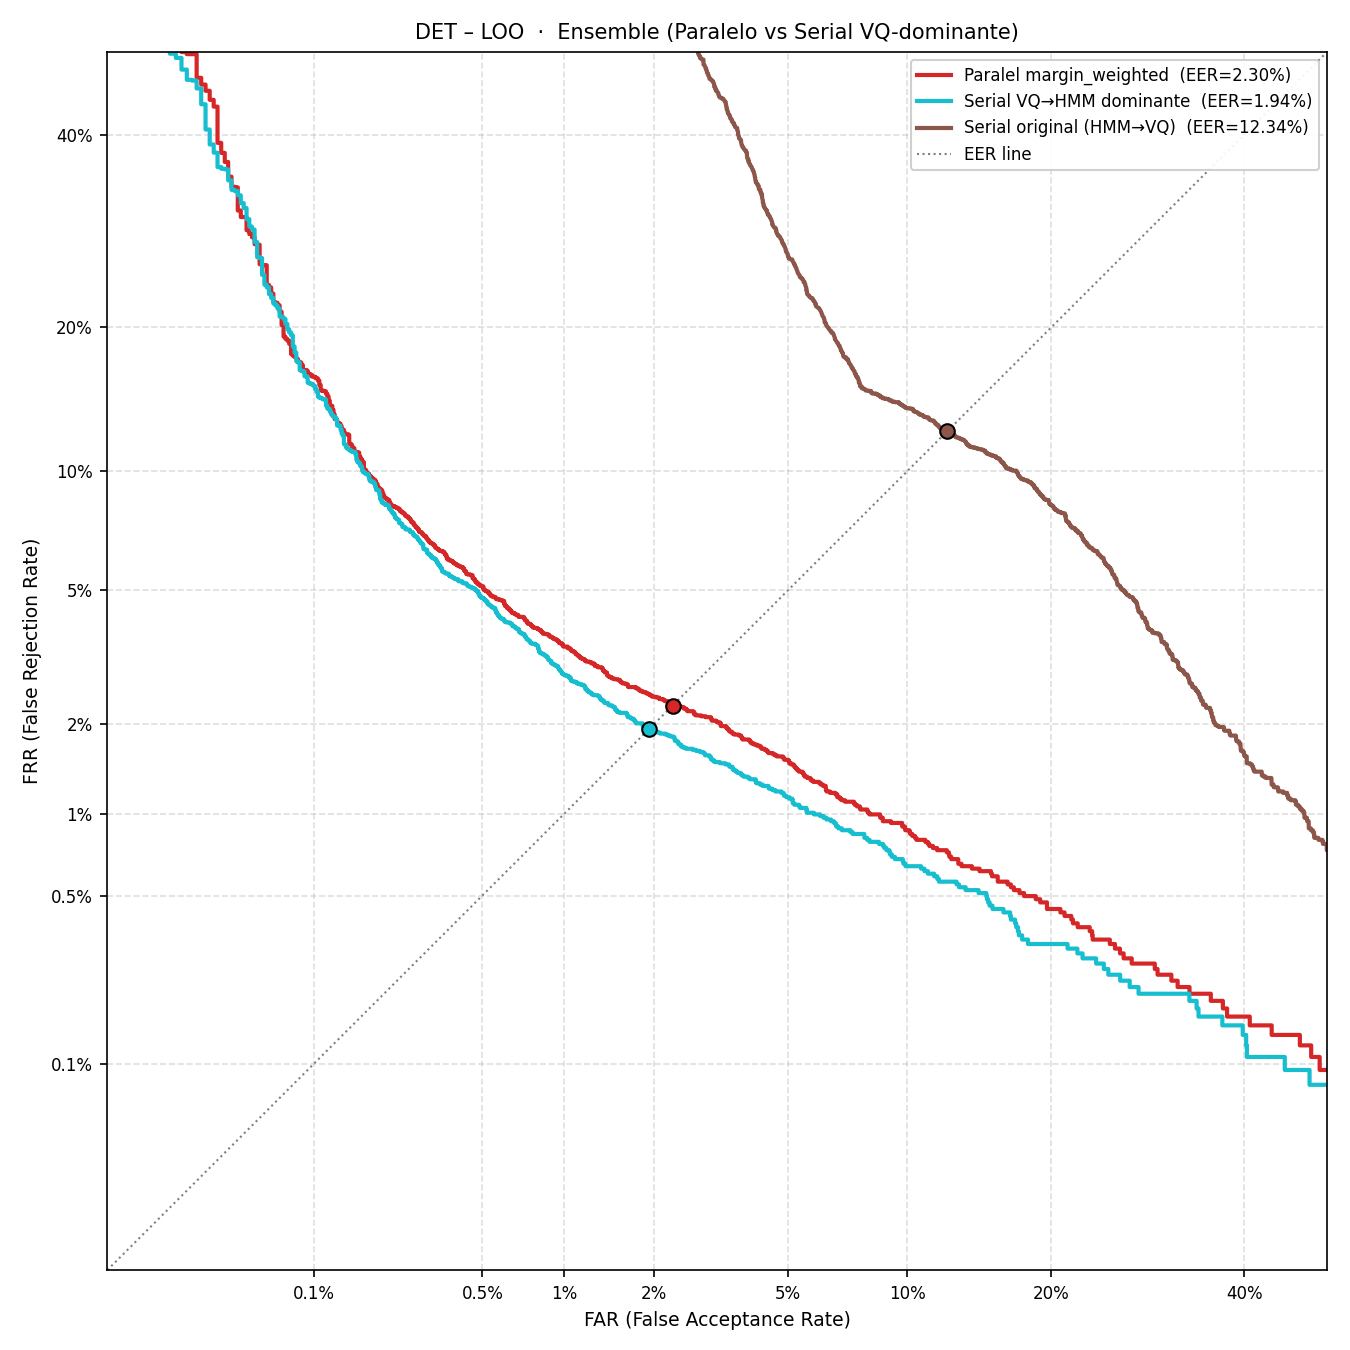
\includegraphics[width=0.65\textwidth, keepaspectratio]{plot3_LOO.png}
  \caption{Curvas DET (LOO): sistemas en ensemble.}
\end{figure}

\subsection{Conclusiones de los ensembles}

Los resultados confirman que combinar HMM y VQ es una buena estrategia. El
ensemble paralelo con \texttt{margin\_weighted} mejora el EER del mejor modelo
individual (VQ opt., 1.90\% en LOO) hasta un 2.30\% en LOO. Este resultado
aparentemente peor en LOO se debe a que el GMMHMM del LOO se entren\'{o} con
par\'{a}metros reducidos (K5-fold, 80 iter., 6 reinicios), lo que limita su
contribuci\'{o}n al ensemble; en los escenarios con entrenamiento completo (N$=$74
y N$=$47) el ensemble s\'{i} mejora al VQ opt.\ de forma clara.

El serial original es un fracaso porque la cadena HMM $\to$ VQ traslada
los errores del HMM al segundo etapa en lugar de corregirlos. La versi\'{o}n
VQ-dominante revierte la direcci\'{o}n de la cascada y conv\'{i}erte al VQ en la
etapa primaria fiable, usando el HMM solo como respaldo. Con este cambio el
serial compite directamente con el paralelo y, en N$=$47, incluso lo supera
ligeramente (1.66\% frente a 1.74\%).

\end{document}
